\usetikzlibrary {shapes.geometric}
\usetikzlibrary{positioning}
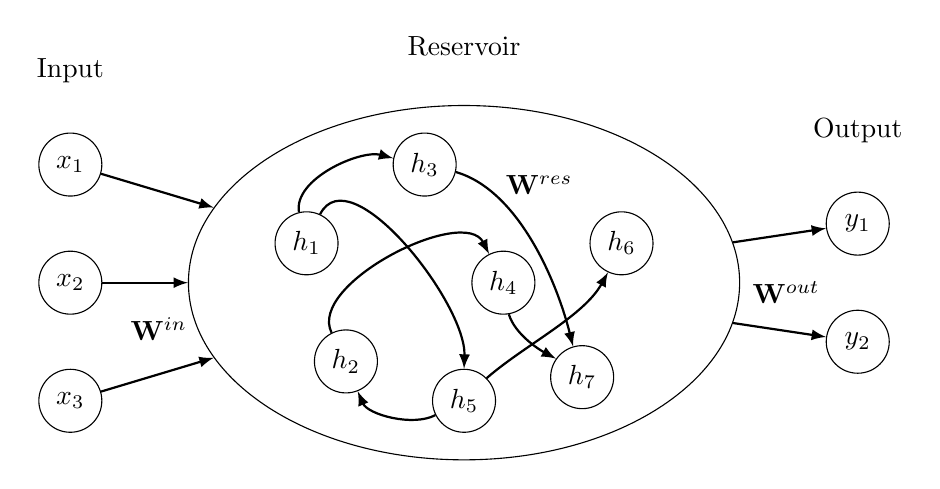
\begin{tikzpicture}[    
    node/.style={draw, circle, minimum size=0.8cm},
    arrow/.style={->, >=latex, thick},
    hidden_layer/.style={draw, ellipse, minimum width=7cm, minimum height=4.5cm}
]

% Input layer
\node[node, label={[label distance=0.5cm]north:Input}] (x1) at (0, 0) {$x_1$};
\node[node] (x2) at (0, -1.5) {$x_2$};
\node[node, label={[label distance=0.5cm]north east:$\mathbf{W}^\text{in}$}] (x3) at (0, -3) {$x_3$};

% Hidden layer
\node[hidden_layer, label={[label distance=0.5cm]north:Reservoir}] (hidden) at (5, -1.5) {};
\node[node] (h1) at (3, -1) {$h_1$};
\node[node] (h2) at (3.5, -2.5) {$h_2$};
\node[node] (h3) at (4.5, 0) {$h_3$};
\node[node] (h4) at (5.5, -1.5) {$h_4$};
\node[node] (h5) at (5, -3) {$h_5$};
\node[node, label={[label distance=0.3cm]north west:$\mathbf{W}^\text{res}$}] (h6) at (7, -1) {$h_6$};
\node[node] (h7) at (6.5, -2.7) {$h_7$};

% Output layer
\node[node, label={[label distance=0.5cm]north:Output}] (y1) at (10, -0.75) {$y_1$};
\node[node, label={[label distance=0.1cm]north west:$\mathbf{W}^\text{out}$}] (y2) at (10, -2.25) {$y_2$};

% Edges
\foreach \i in {1,2,3}
    \draw[arrow] (x\i) -- (hidden);

\foreach \j in {1,2}
    \draw[arrow] (hidden) -- (y\j);

% Recurrent connections
\draw[arrow, bend right] (h1) to[out=70,in=135,looseness=0.8] (h3);
\draw[arrow, bend right] (h1) to[out=110,in=135,looseness=0.8] (h5);
\draw[arrow, bend right] (h2) to[out=90,in=90,looseness=0.8] (h4);
\draw[arrow, bend right] (h3) to[out=40,in=160,looseness=0.8] (h7);
\draw[arrow, bend right] (h4) to[out=330,in=195,looseness=0.8] (h7);
\draw[arrow, bend right] (h5) to[out=0,in=200,looseness=0.8] (h6);
\draw[arrow, bend right] (h5) to[out=45,in=130,looseness=0.8] (h2);

\end{tikzpicture}
